\section{Frontend}
\subsection{Technologies and libraries}
\subsubsection{NextJS}
NextJS is an open-source\textsubscript{\textbf{G}} React framework\textsubscript{\textbf{G}} created by Vercel. It supports TypeScript, static generation\textsubscript{\textbf{G}} and server-side rendering\textsubscript{\textbf{G}} which improves the site's search engine optimization. It also supports dynamic routing of pages.
\begin{itemize}
  \item \textbf{Used Version: 10.2}
  \item \textbf{Link: \url{https://nextjs.org/}}
\end{itemize}
\subsubsection{React}
React is an open-source\textsubscript{\textbf{G}}, frontend, Javascript library for building user interfaces, maintained by Facebook. It's component based and it supports TypeScript. Since is made for single-page development additional libraries are required for routing.
\begin{itemize}
  \item \textbf{Used Version: 17.0.3}
  \item \textbf{Link: \url{https://reactjs.org/}}
\end{itemize}
\subsubsection{Chakra UI}
Chakra UI is a React component library made with TypeScript and NextJS in mind. It is accessible and flexible, makes the styling fast and easy.
\begin{itemize}
  \item \textbf{Used Version: 1.6.1}
  \item \textbf{Link: \url{https://chakra-ui.com/}}
\end{itemize}
\subsubsection{NextAuth}
NextAuth.js is a complete open source authentication solution for Next.js applications. It is designed from the ground up to support Next.js and Serverless.
\begin{itemize}
  \item \textbf{Used Version: 3.14.8}
  \item \textbf{Link: \url{https://next-auth.js.org/}}
\end{itemize}
\subsubsection{Swiper}
Swiper is a React componenent that render a touch slider with hardware accelerated transitions.
\begin{itemize}
  \item \textbf{Used Version: 6.7.0}
  \item \textbf{Link: \url{https://swiperjs.com/}}
\end{itemize}
\subsubsection{Cookies}
Cookies is a node.js module for getting and setting HTTP(S) cookies.
\begin{itemize}
  \item \textbf{Used Version: 0.8.0}
  \item \textbf{Link: \url{https://www.npmjs.com/package/cookies}}
\end{itemize}
\subsubsection{Jest}
Jest is a JavaScript testing framework designed to ensure correctness of any JavaScript codebase.
\begin{itemize}
  \item \textbf{Used Version: 27.0.6}
  \item \textbf{Link: \url{https://jestjs.io/docs/getting-started}}
\end{itemize}

\subsection{General description}
The frontend\textsubscript{\textbf{G}} structure has three macro categories that explains its works:
\begin{itemize}
  \item data fetching;
  \item components;
  \item the npm package \textit{utilities-techsweave}.
\end{itemize}

This is a package diagram to show the principal architecture of \textit{EmporioLambda} and his principal part.
\begin{figure}[!ht]
  \caption{Frontend package diagram}
  \vspace{10px}
  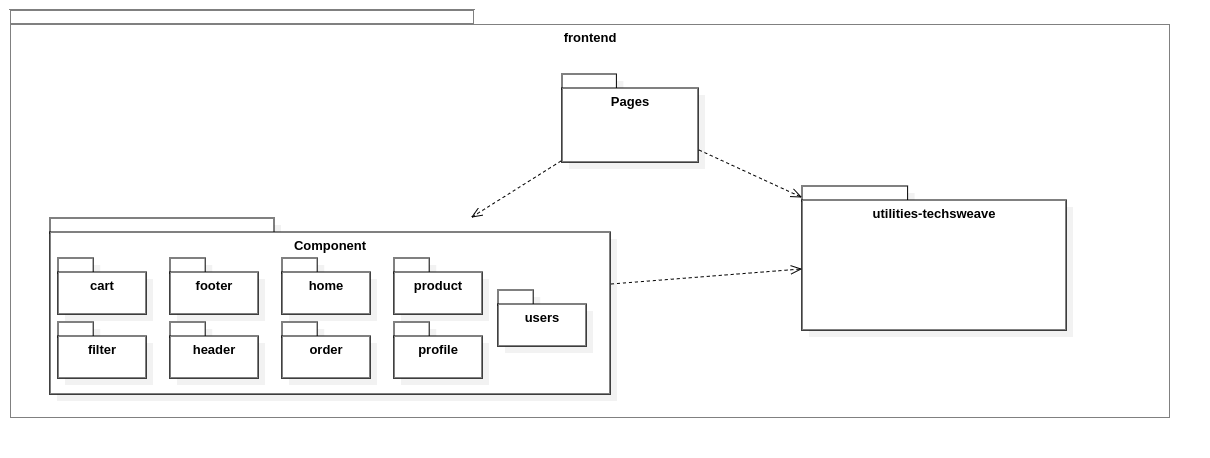
\includegraphics[scale=0.39]{../../../../Images/Diagrammi/maintainerManual/FE/FEgraph.png}
  \centering
\end{figure}

\subsubsection{Data fetching}
For the data fetching we followed the \textit{Next.js} and \textit{React} best paractices.
\\
\\
\textit{Next.js} for the data fetching pre-renders every page. This means that \textit{Next.js} generates HTML for each page in advance, instead of having it all done by client-side \textit{JavaScript}. Next offers two type of pre-rendering:
\begin{itemize}
  \item \textbf{Static Generation:} The HTML is generated at build time and will be reused on each request;
  \item \textbf{Server-side Rendering}: The HTML is generated on each request.
\end{itemize}
Static generation performs significantly better than Server-side Rendering this because with static generation a page can be cached in the server and every time the browser need it the server just send the page without rebuilding it. For this reason we choose to use static generation in all pages that are directly addressed by browser, beacuse the page are always shown entirely to the browser and this allows better SEO perfomances. Some pages can't be generated with static generetion, because their data has to be constantly and rapidly update or because there is sessione verification to allow access to the page.
\\
\\
We also use \textit{React} data fetching method, that consists in a client side rendering that allows to have some preformace benefits.
Every page of \textit{EmporioLambda} fetches data using this method:
\begin{itemize}
  \item \textbf{getStaticProps:} a function that returns a GetStaticProps object, which indicates that the page will use static generation;
  \item \textbf{getServerSideProps:} a function that return a GetServerSideProps object, which indicates that the page will use server-side renderingG. It will  re-render the page after receiving new data, or at evrey request.
  \item \textbf{useEffect:} a \textit{React} function which consists of modify parts of the pages when needed.
\end{itemize}
\subsubsection{Components}
\textit{EmporioLambda} use \textit{React}, \textit{JavaScript} and \textit{TypeScript} to use components. Components are HTML snippets that allow us to create the UI and its parts. The usign of components allowed us to separate the business logic from the presentation logic. In \textit{EmporioLambda} has two type components:
\begin{itemize}
  \item \textbf{presentation components:} these components has the only scope to render the data fetched from pages. This type of components can only call other presentation components;
  \item \textbf{container components:} these components can use state and function to fetch or send data to the business logic. These type of components can also call presentation components sending to them the needed data.
\end{itemize}
The \textit{React} components can accept two different variables:
\begin{itemize}
  \item \textbf{Props:} variables or object that can only be passed from a parent component to a children component. Props can be used from a next page so give to his principal component the needed data.
  \item \textbf{State:} these variables cause the re-rendering of a component. This state has to be initialized from the component constructor.
\end{itemize}
The use of state variables allows us to introduce the \textit{Observer pattern} a design pattern used by the frontend to render a page. This design pattern is native implmented in \textit{React}. In our case the state of the component is our observable: the component, when the state has been changed, automatically re-renders the page with the new values, re-rendering its children as well.
\\
\\
The following diagrams show the structure of every page.
\begin{figure}[!ht]
  \caption{ Frontend homepage component diagram}
  \vspace{10px}
  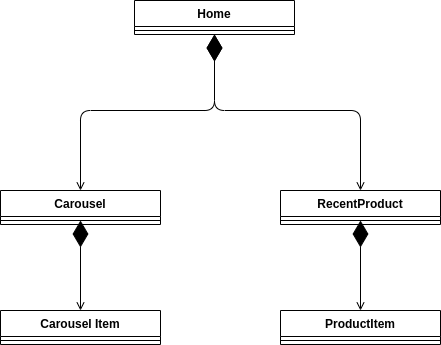
\includegraphics[scale=0.39]{../../../../Images/Diagrammi/maintainerManual/FE/HomeDiagram.png}
  \centering
\end{figure}
\begin{figure}[!ht]
  \caption{ Frontend product listing page component diagram}
  \vspace{10px}
  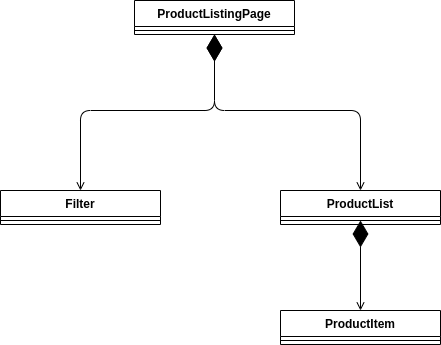
\includegraphics[scale=0.39]{../../../../Images/Diagrammi/maintainerManual/FE/PLPDiagram.png}
  \centering
\end{figure}
\begin{figure}[!ht]
  \caption{ Frontend product detail page component diagram}
  \vspace{10px}
  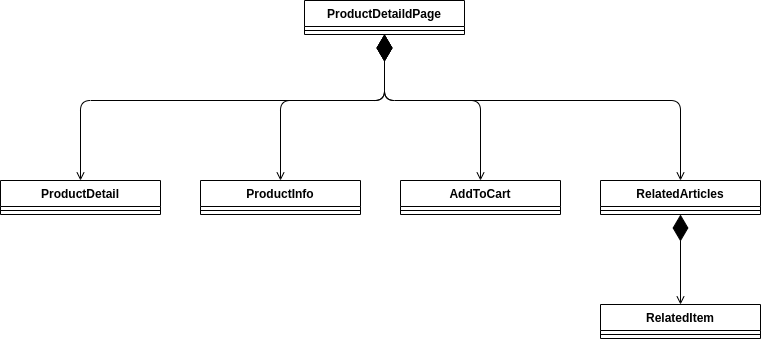
\includegraphics[scale=0.39]{../../../../Images/Diagrammi/maintainerManual/FE/PDPDiagram.png}
  \centering
\end{figure}
\begin{figure}[!ht]
  \caption{ Frontend cart page component diagram}
  \vspace{10px}
  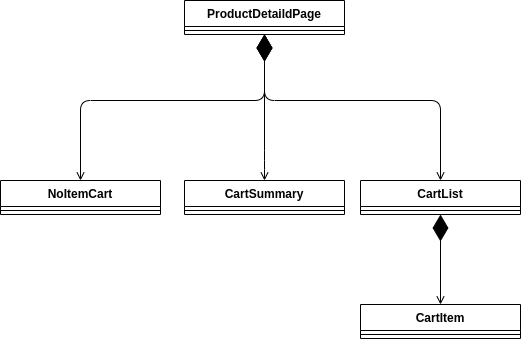
\includegraphics[scale=0.39]{../../../../Images/Diagrammi/maintainerManual/FE/CartDiagram.png}
  \centering
\end{figure}
\begin{figure}[!ht]
  \caption{ Frontend profile page component diagram}
  \vspace{10px}
  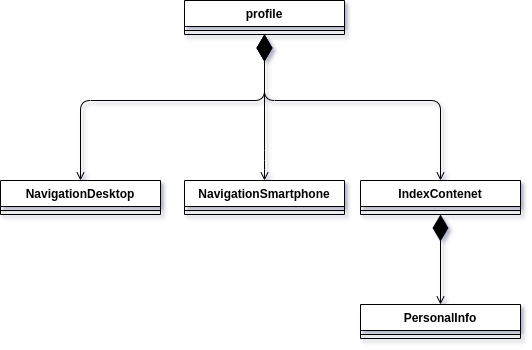
\includegraphics[scale=0.39]{../../../../Images/Diagrammi/maintainerManual/FE/ProfileDiagram.png}
  \centering
\end{figure}
\begin{figure}[!ht]
  \caption{ Frontend edit profile page component diagram}
  \vspace{10px}
  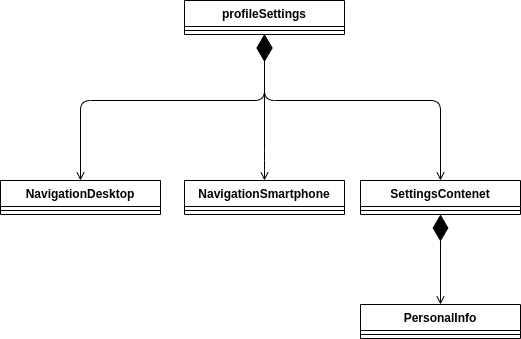
\includegraphics[scale=0.39]{../../../../Images/Diagrammi/maintainerManual/FE/EditProfileDiagram.png}
  \centering
\end{figure}
\begin{figure}[!ht]
  \caption{ Frontend order page component diagram}
  \vspace{10px}
  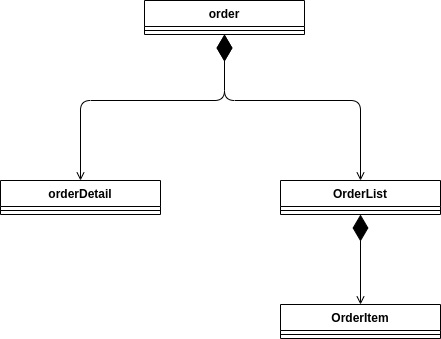
\includegraphics[scale=0.39]{../../../../Images/Diagrammi/maintainerManual/FE/orderDiagram.png}
  \centering
\end{figure}
\begin{figure}[!ht]
  \caption{ Frontend edit product page component diagram}
  \vspace{10px}
  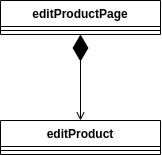
\includegraphics[scale=0.39]{../../../../Images/Diagrammi/maintainerManual/FE/editProductDiagram.png}
  \centering
\end{figure}
\begin{figure}[!ht]
  \caption{ Frontend manage shop page component diagram}
  \vspace{10px}
  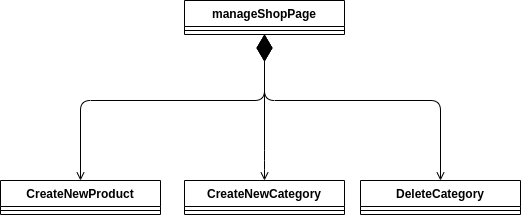
\includegraphics[scale=0.39]{../../../../Images/Diagrammi/maintainerManual/FE/manageShopDiagram.png}
  \centering
\end{figure}
\clearpage
\subsubsection{Utilities-techsweave}
\textit{Utilities-techsweave} is a npm package which has the same function as a library. Especially the package provides to the frontend all types and services made from the backend. Thanks to this package we have been able to greatly simplify interactions between frontend and backend, in fact the implementation of the method is trasparent to the frontend, the only thing that frontend knows about the method is its signature.
In addition to methods \textit{utilities-techsweave} provides type used in the various function, in this case the frontend module has only to create e new type based on what the package provides. With this package the separetion of presentation logic and buisness logic it's further accentuated thus allowing to the frontend to focus on the presentation logic. This marked separetion of concepts consists in a better stability for the finished.















\subsection{Examples of functioning}
\subsubsection{Use of a function}
To call a method exposed from \textit{utilities-techsweave}, first we have to import Module and Services from utilities-techsweave in the file.
\begin{lstlisting}
    import { Models, Services } from 'utilities-techsweave'
\end{lstlisting}
After this we have to create a new istance of the type that we want to use in the page, for example if we need a scan of the product we have to create a new istance of {\fontfamily{qcr}\selectfont IProduct}. This type istance is the caller for the method that we want to use, following the previous example the caller allows us to call the {\fontfamily{qcr}\selectfont scanAsync} method that return the scan of product's table in the DB. This procedure has to be done inside the fetch function previously explained:
\begin{itemize}
  \item {\fontfamily{qcr}\selectfont getStaticProps}
  \item {\fontfamily{qcr}\selectfont getServerSideProps}
  \item {\fontfamily{qcr}\selectfont useEffect and an async function}
\end{itemize}
\subsubsection{Rendering of a page}
The rendering of page  is a succession of components calls. All starts from the page that include and call some components and does the data fetching. When the page has the data, passes it to the component. The \textit{Layout} component contains the general style of the page including header, footer and navbar, and it's included in every page. The product detail page renderign has the following procedure:
\begin{itemize}
  \item \textbf{ProductDetail} is the main component this component takes care of showing the data of the product like, his title, his image and his price, and calls all other components:
        \begin{itemize}
          \item \textbf{RelatedProduct}, creates a list of products with the same category of the one currently displayed, to achieve this the component calls the RelatedItem that render the single item of the list ;
          \item \textbf{ProductInfo}, creates a list of products specifications;
          \item \textbf{AddToCart}, displays a button to add the currently displayed product in the cart.
        \end{itemize}
\end{itemize}

